% - How to build the CRT
\section{The Cosmic Ray Tagger}
Detecting and tracing incident ionizing background radiation to distinguish background from a \gls{bnb}-based event in the \gls{lartpc} is the main goal of the \gls{crt}.
This section covers the \gls{crt} modules functionality and important parameters are listed.

\subsection{The Cosmic Ray Tagger in a nutshell}
If the times and positions at which an incident particle entered and exited our detector are known, we can identify the crossing particle's trace.
To trace incident radiation in a \gls{tpc}, the latter needs to be covered with an additional detector generating a grid.
This additional detector is the \gls{crt} and a scheme of it is illustrated in figure \ref{fig:scheme}.

\begin{figure}
  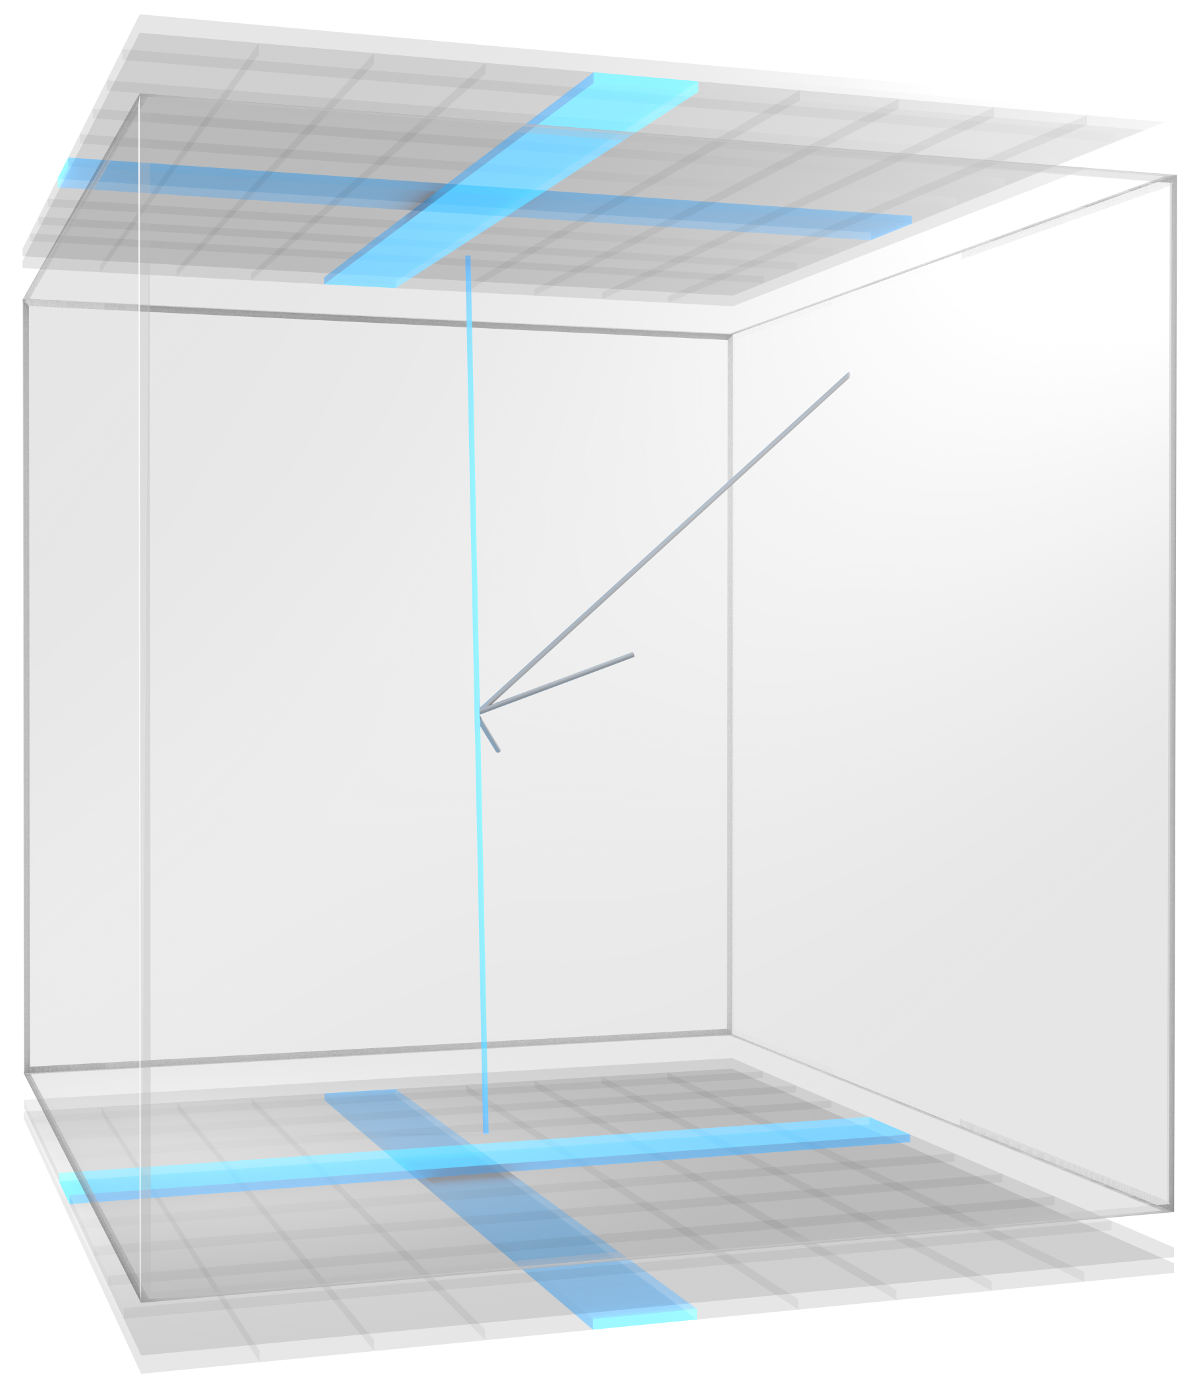
\includegraphics[width=.9\textwidth]{detector}
  \caption{%
    Schematic of two layers of \gls{crt} positioned above and below a virtual \gls{tpc} containing an event.
    The event represents the interaction between a muon neutrino and a proton ($\nu_\mu + p \to p' + \pi^+ + \mu$) with an atmospheric muon travelling close to the event's vertex.
    The highlighted scintilating bars are crossed by the atmospheric muon.
    Using the grid produced by the scintilating bars the atmospheric muon's path can be identified.
  }
  \label{fig:scheme}
\end{figure}

The \gls{crt} consists of several independent detectors (modules), making it fully modulable.
Each \gls{crt} module consists of a \gls{crt} panel and a \gls{feb}, which processes the panel's incoming signals to event data.
A layer of \gls{crt} requires at least two panels -- to generate a grid of scintillating pixels -- and two layers are needed to track incident particles.
If the position of the panels is well known, their signals and time coincidence can be used to determine the entry and exit points of the incident particle.

\subsection{Background mitigation}

Charged particles will generate a signal in our \gls{crt} modules.
Using these signals, a cylindrical volume can be constructed around the path of the incident particles.
This volume acts as a veto for the track.

If the vertex of a neutrino event is inside the veto region, the event needs to be reconstructed with more delicate algorithms to distinguish the neutrino signal from the cosmic signal.
The following parameters of the detector are of severe importance to achieve a useful veto signal with the smallest possible volume..

\paragraph{Time resolution} The time a particle takes to cross our detector is given by the particle's velocity.
If the \gls{crt} modules are run without using the coincidence signals featured by the \gls{feb}, these coincidences need to be reconstructed from the detector data.
A precise time resolution is required for this task.

\paragraph{Position resolution} is principally given by the width of the bars installed in the module.
This resolution can be improved by calibrating the signal ratio and signal amplitudes for the channels of a bar.

\paragraph{Detection efficiency} Not every occurrent particle transition is registered as an event by our detector.
Many physical effects\marginnote{Quantum efficiencies, geometrical fill factors, surface reflections, detection ranges, signal losses\ldots} influence the particle detection efficiency of the \gls{crt}.
An important contribution to detection efficiency is made by the set threshold, since it will change the part of the energy spectrum observed by the \gls{crt}.
